\documentclass[a4paper,11pt,cours]{nsi} % COMPILE WITH DRAFT
\geometry{margin=2cm}
\usepackage[]{fontawesome5}
\usepackage{pgfplots}
\usepackage{hyperref}


\setcounter{chapter}{5} % 1 de moins que le num de chapitre

\setlength{\columnseprule}{0pt}
\setlength{\columnsep}{1cm}

\chapter{Statistiques à deux variables quantitatives}

\begin{document}

\section{Nuage de points et ajustement affine}

\subsection*{Série statistique à deux variables quantitatives}
Sur une population, on étudie deux caractères quantitatifs $x$ et $y$ (par exemple l'ancienneté et la prime d'un employé). Pour chacun des $n$ individus de cette population, on note $x_i$ et $y_i$ les valeurs prises par chacun de ces deux caractères et on présente les données à l'aide de la \textbf{série statistique à deux variables} ci dessous :

\begin{center}
    \tabstyle[UGLiBlue]
    \begin{tabular}{|c|c|c|c|c|}
    \hline
    \ccell valeur $x_i$ & $x_1$ & $x_2$ & ... & $x_n$ \\\hline
    \ccell Valeur $y_i$ & $y_1$ & $y_2$ & ... & $y_n$ \\\hline
    \end{tabular}
\end{center}

\begin{definition}[s]
    \begin{enumerate}[label=\textbullet]
        \item Dans un repère, le $\textbf{nuage de points}$ associé à cette série statistique est l'ensemble des points $\pc{M_i}{x_i}{y_i}$ pour $i=1,2,...,n$.
        \item Le \textbf{point moyen} de cette série statistique est le point $\pc{M}{\overline{x}}{\overline{y}}$ où $\overline{x}=\dfrac{x_1+x_2+...+x_n}{n}$ et $\overline{y}=\dfrac{y_1+y_2+...+y_n}{n}$.
    \end{enumerate}
\end{definition}

\subsection*{Ajustement d'un nuage de points}
On se demande s'il existe une dépendance entre les deux caractères $x$ et $y$.
\begin{multicols}{3}
    Figure 1\\
    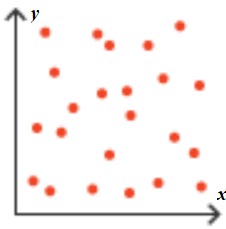
\includegraphics[width=3cm]{Figure3.png}\\
    Figure 2\\
    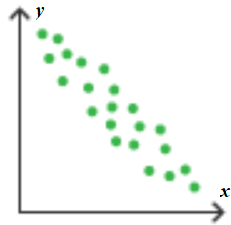
\includegraphics[width=3cm]{Figure1.png}\\
    Figure 3\\
    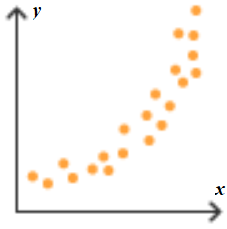
\includegraphics[width=3cm]{Figure2.png}
\end{multicols}

Selon la forme du nuage associé, on peut être incité à ne pas voir de dépendance (figure 1), ou bien à penser que les points se répartissent autour d'une droite (figure 2), ou bien autour d'un autre type de courbe (figure 3).

\begin{definition}[]
    Pratiquer un \textbf{ajustement affine} d'un nuage de point consiste à tracer une droite qui passe le plus près possible des points du nuage.\\
\end{definition}

On se demande :
\begin{enumerate}[label=\textbullet]
    \item Quelle droite tracer ?
    \item Y-en-a-t-il une meilleure que les autres ?
    \item Meilleure... selon quel critère ?
\end{enumerate}

\begin{exemple}[]
    On reprend l'exemple des employés du service informatique. On considère la série statistique à deux variables suivante :
    \begin{center}
        \tabstyle[UGLiBlue]
        \begin{tabular}{|c|c|c|c|c|c|c|}
        \hline
        \ccell $x_i$ & 2 & 8 & 11 & 17 & 20 & 22 \\\hline
        \ccell $y_i$ & 290 & 390 & 450 & 580 & 640 & 710 \\\hline
        \end{tabular}
    \end{center}
    On représente le nuage de points associé dans un repère orthonormé.\\
    \begin{center}
        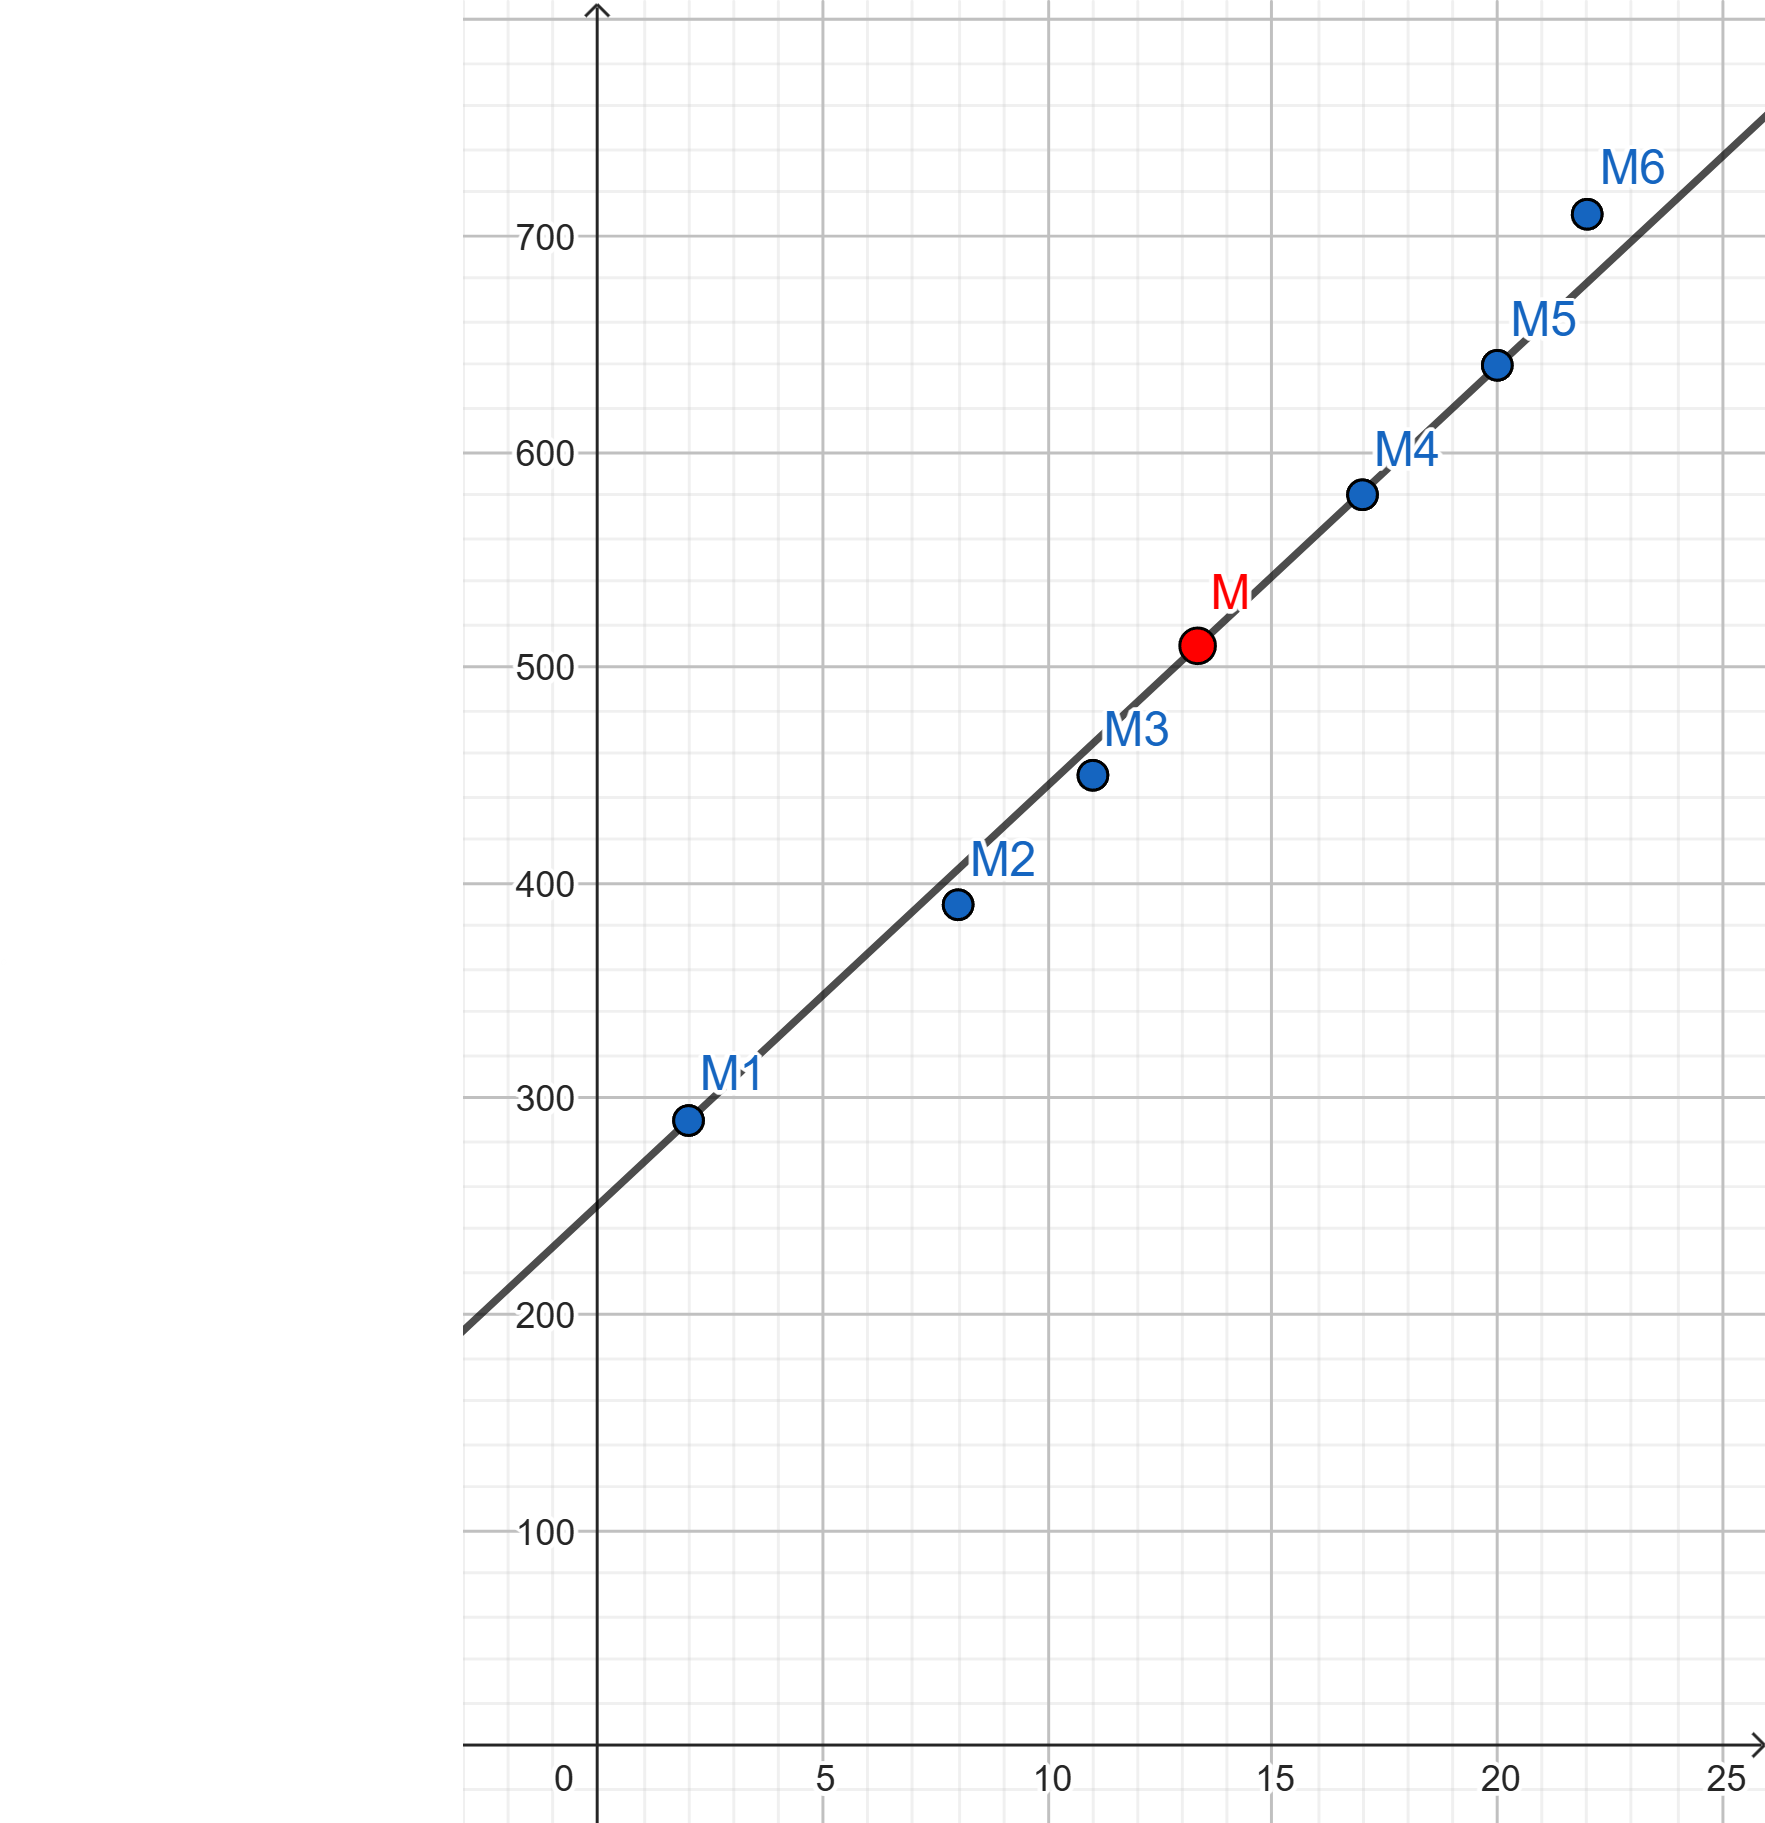
\includegraphics[width=10cm]{Ajustement1.png}
    \end{center}
    Le point moyen du nuage de points est $\pc{M}{\overline{x}}{\overline{y}}$ où :
    \begin{align*}
        \overline{x} &= \dfrac{2+8+11+17+20+22}{6} \approx 13,33\\
        \overline{y} &= \dfrac{290+390+450+580+640+710}{6} = 510
    \end{align*}
    Le nuage de point a une forme alongée, on peut l'ajuster par exemple par la droite $(MM_1)$.
\end{exemple}

\section{Droite des moindres carrés}

\begin{encadrecolore}{Principe de la méthode des moindres carrés}{UGLiDarkBlue}
    Le principe de l'ajustement consiste à estimer les coefficients $m$ et $p$ de la droite d'équation $y=mx+p$ qui passe le plus près possible des points du nuage.\\
    \dleft{7cm}{
        Pour cela, on cherche à minimiser la somme des carrés des distances entre les points du nuage et la droite.\\
    Ainsi les nombres réels $m$ et $p$ sont choisis de sorte que la somme suivante soit minimale :
    $$\sum_{i=1}^n M_iA_i^2=\sum_{i=1}^n \left(y_i-(mx_i+p)\right)^2$$
    }
    {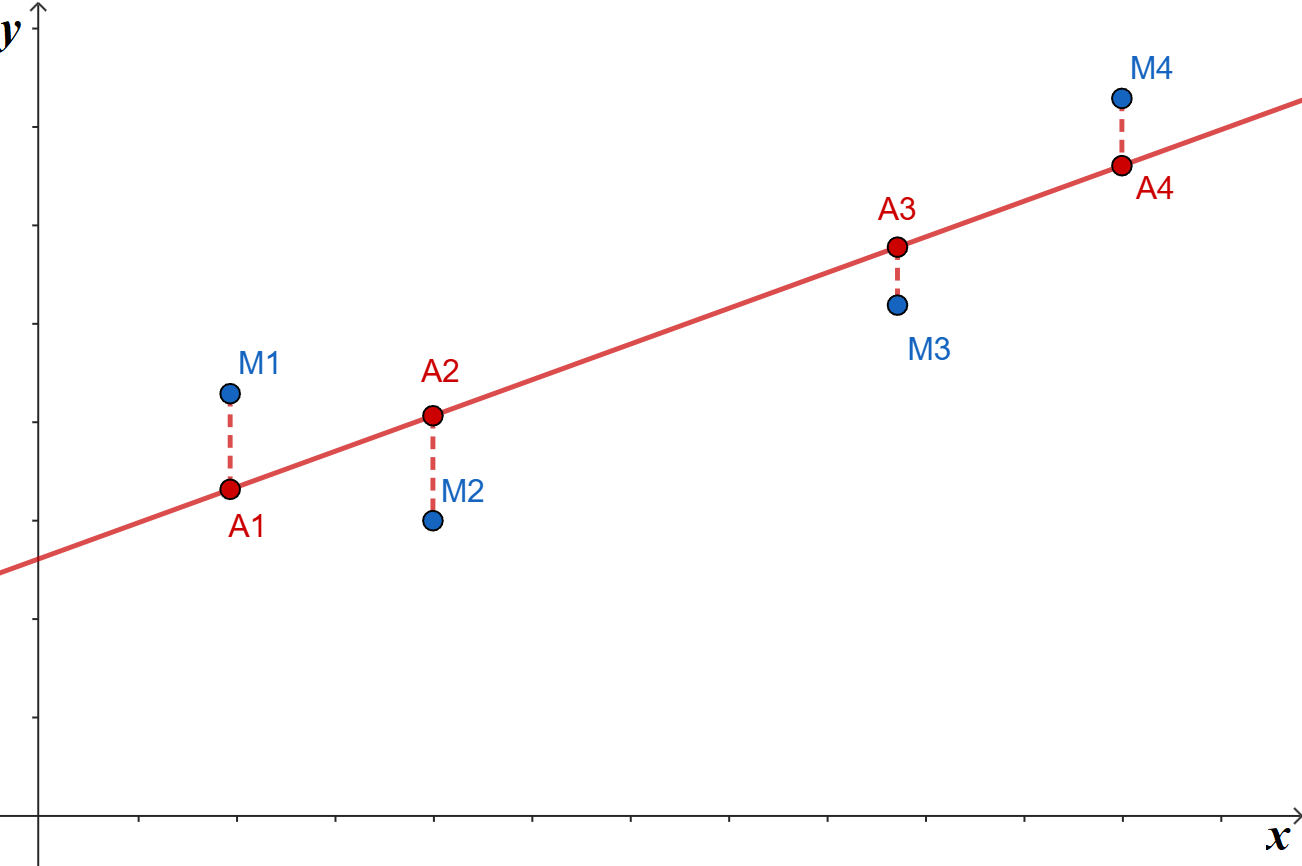
\includegraphics[width=8.5cm]{Moindre_carres.png}} 
\end{encadrecolore}

\begin{definition}[s]
    Soient $(x_i)$ et $(y_i)$ deux séries statistiques composées de $n$ valeurs.\\
    On note $\overline{x}$ et $\overline{y}$ les moyennes de ces deux séries.\
    \begin{enumerate}[label=\textbullet]
        \item La \textbf{variance} de la série $(x_i)$ est : $\displaystyle \quad V(x)=\dfrac{1}{n}\sum_{i=1}^n (x_i-\overline{x})^2$ ;\\
        La \textbf{variance} de la série $(y_i)$ est : $\displaystyle \quad V(y)=\dfrac{1}{n}\sum_{i=1}^n (y_i-\overline{y})^2$
        \item L'\textbf{écart-type} de la série $(x_i)$ est : $\displaystyle \quad \sigma_x=\sqrt{V(x)}$\\[.5em]
        L'\textbf{écart-type} de la série $(y_i)$ est : $\displaystyle \quad \sigma_y=\sqrt{V(y)}$
        \item La \textbf{covariance} de la série $(x_i;y_i)$ est :
        $\quad \displaystyle \mathrm{Cov}(x,y)=\dfrac{1}{n}\sum_{i=1}^n (x_i-\overline{x})(y_i-\overline{y})$.
    \end{enumerate}
\end{definition}

\begin{propriete}[ (admise)]
    Dans un repère orthonormé, la droite des moindres carrés associée au nuage de points $\pc{M_i}{x_i}{y_i}$ :
    \begin{enumerate}[label=\textbullet]
        \item passe par le point moyen $\pc{M}{\overline{x}}{\overline{y}}$ ;
        \item a pour équation $\quad y=m(x-\overline{x})+\overline{y}\quad$ avec $\quad m=\dfrac{\mathrm{Cov}(x,y)}{V(x)}$.
    \end{enumerate}
\end{propriete}

\begin{remarque}[s]
    \begin{enumerate}[label=\textbullet]
        \item On peut obtenir les coefficients $m$ et $p$ de la droite des moindres carrés à l'aide du menu « Régressions » de la calculatrice.
        \item La covariance $\mathrm{Cov}(x,y)$ peut être positive ou négative. On la note aussi $\sigma_{xy}$.
    \end{enumerate}
\end{remarque}


\begin{demonstration}
    \begin{tabbing}
        $S$ \= $=\displaystyle \sum_{i=1}^n A_iM_i^2$ \\
        \> $=\displaystyle \sum_{i=1}^n \left(y_i-(mx_i+p)\right)^2$\\
        \> $=\displaystyle \sum_{i=1}^n \left((y_i-mx_i)-p\right)^2 \qquad$ (*)\\
        \> $=\displaystyle \sum_{i=1}^n \left((y_i-mx_i)^2-2p(y_i-mx_i)+p^2\right)$\\
        \> $=\displaystyle \sum_{i=1}^n (y_i-mx_i)^2-2p\sum_{i=1}^n (y_i-mx_i)+ \sum_{i=1}^np^2$\\
        \> $=\displaystyle \sum_{i=1}^n (y_i-mx_i)^2-2p\sum_{i=1}^n (y_i-mx_i)+np^2$
    \end{tabbing}
    \begin{enumerate}[label=\textbullet]
        \item On suppose que $m$ est fixé.\\
        $S$ est donc un polynôme du second degré en $p$ de la forme $S(p)=ap^2+bp+c$ avec $a=n$.\\
        $a>0$ donc $S$ admet un minimum atteint lorsque sa dérivée s'annule.
        \begin{tabbing}
            $S'(p)=0\quad$ \= $\iff \quad \displaystyle 2np-2\sum_{i=1}^n (y_i-mx_i)=0$\\
            \> $\iff \quad \displaystyle p=\dfrac{1}{n}\sum_{i=1}^n (y_i-mx_i)$\\
            \> $\iff \quad \displaystyle p=\dfrac{1}{n}\sum_{i=1}^n y_i-\dfrac{m}{n}\sum_{i=1}^n x_i$\\
            \> $\iff \quad \displaystyle p=\overline{y}-m\overline{x}$
        \end{tabbing}

        \begin{tabbing}
            Donc $\quad S$  \=$=\displaystyle \sum_{i=1}^n \left(y_i-mx_i-\overline{y}+m\overline{x}\right)^2 \qquad$ d'après (*)\\
            \> $=\displaystyle \sum_{i=1}^n \left((y_i-\overline{y})-m\left(x_i-\overline{x}\right)\right)^2$\\
            \> $=\displaystyle \sum_{i=1}^n \left((y_i-\overline{y})^2-2m(y_i-\overline{y})(x_i-\overline{x})+m^2(x_i-\overline{x})^2\right)$\\
            \> $=\displaystyle \sum_{i=1}^n (y_i-\overline{y})^2-2m\sum_{i=1}^n (y_i-\overline{y})(x_i-\overline{x})+m^2\sum_{i=1}^n (x_i-\overline{x})^2$\\
            \> $=\displaystyle nV(y)-2mn \mathrm{Cov}(x,y)+m^2nV(x)$
        \end{tabbing}

        \item $S$ est donc un polynôme du second degré en $m$ de la forme $S(m)=am^2+bm+c$ avec $a=nV(x)>0$. Il admet donc un minimum atteint lorsque sa dérivée s'annule.
        \begin{tabbing}
            $S'(m)=0\quad$ \= $\iff \quad \displaystyle 2nV(x)m-2n\mathrm{Cov}(x,y)=0$\\
            \> $\iff \quad \displaystyle m=\dfrac{\mathrm{Cov}(x,y)}{V(x)}$
        \end{tabbing}
        \item On en déduit que la droite des moindres carrés a pour équation réduite :
        $$y=mx+\overline{y}-m\overline{x}=m(x-\overline{x})+\overline{y}$$
    \end{enumerate}
\end{demonstration}



\section{Coefficient de corrélation. Changement de variable}

\subsection*{Coefficient de corrélation linéaire}

La décision d'ajuster un nuage de points par une droite s'est prise jusqu'à présent à la seule vue du nuage de points (suivant que celui-ci est allongé ou non).\\
Les statisticiens ont mis au point un coefficient de corrélation linéaire qui permet de quantifier la dépendance entre deux caractères quantitatifs.

\begin{definition}[]
    Le \textbf{coefficient de corrélation linéaire} entre les deux séries $(x_i)$ et $(y_i)$ est le nombre réel noté $r$ et défini par :
    $$r=\dfrac{\mathrm{Cov}(x,y)}{\sigma_x \sigma_y}$$
\end{definition}

\begin{propriete}[]
    Pour toute série statistique à deux variables quantitatives, on a : $\quad -1\leq r \leq 1$.
    \begin{enumerate}[label=\textbullet]
        \item plus $|r|$ est proche de 1, plus la dépendance entre les deux caractères est forte ;
        \item plus $|r|$ est proche de 0, plus la dépendance entre les deux caractères est faible ;
        \item si $|r|=1$, les points du nuage de points sont alignés sur une droite ;
        \item si $r>0$, la droite a une pente positive (la variable $y$ augmente quand la variable $x$ augmente) ;
        \item si $r<0$, la droite a une pente négative.
    \end{enumerate}
\end{propriete}

%\vspace*{.5cm}

\begin{remarque}[ : Corrélation n'implique pas causalité]
    Une très forte corrélation peut exister entre deux variables sans qu'il y ait de relation de cause à effet entre elles.\\
    Plusieurs exemples \href{https://www.lemonde.fr/les-decodeurs/article/2019/01/02/correlation-ou-causalite-brillez-en-societe-avec-notre-generateur-aleatoire-de-comparaisons-absurdes_5404286_4355770.html}{sur le site des décodeurs du Monde}.
    \begin{center}
        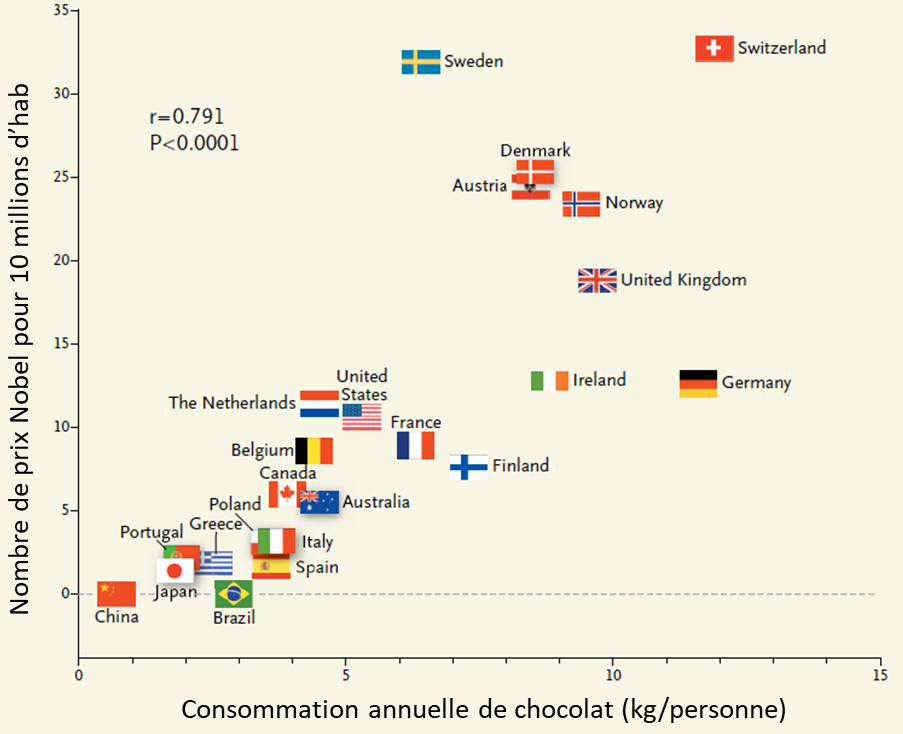
\includegraphics[width=10cm]{Chocalat_prix_Nobel.png}
    \end{center}
\end{remarque}




\subsection*{Ajustement se ramenant par changement de variable à un ajustement affine}
Dans certains cas, les points du nuage de point semblent se répartir autour d'une courbe autre qu'une droite. Il est parfois possible de se ramener à un ajustement affine à l'aide d'un changement de variable.



\begin{multicols}{2}
    \begin{center}
        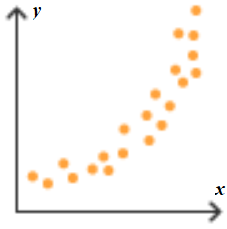
\includegraphics[width=3cm]{Figure2.png}
    \end{center}
    Dans un tel cas, on peut penser qu'il existe une relation du type $y=ax^2+b$ entre $x$ et $y$.\\
    En posant $u=x^2$, on se ramène à $y=au+b$ et on peut déterminer $a$ et $b$ avec la méthode des moindres carrés.\\

    \begin{center}
        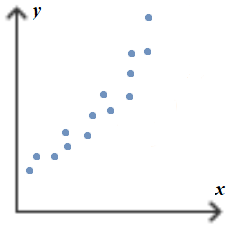
\includegraphics[width=3cm]{Figure4.png}
    \end{center}
    Dans ce cas, on peut penser qu'il existe une relation du type $y=ae^x+b$ entre $x$ et $y$.\\
    En posant $u=e^x$, on se ramène à $y=au+b$ et on peut déterminer $a$ et $b$ avec la méthode des moindres carrés.\\
\end{multicols}
\end{document}